\documentclass{beamer}

\usepackage[T1]{fontenc}
\usepackage[utf8]{inputenc}
\usepackage[slovene]{babel}
\usepackage{etoolbox}
\usepackage{algorithm2e}


\mode<presentation>
{
  \usetheme{Berlin}
  \setbeamercovered{transparent}
}

\makeatletter
\appto\verbatim@font{\footnotesize}
\makeatother

\setbeamertemplate{navigation symbols}{}

\newcommand{\bx}{\mathbf{x}}
\DeclareMathOperator{\Gl}{Gl}
\DeclareMathOperator{\adj}{adj}
\newtheorem{proposition}[theorem]{Proposition}

\title[Paralelizacija grafovskih algoritmov v funkcijskih jezikih]
{Paralelizacija grafovskih algoritmov v funkcijskih jezikih}

\author[Avtor: Tjaž Eržen, Mentor: doc. dr. Matija Pretnar]
{Avtor: Tjaž Eržen\\Mentor: doc. dr. Matija Pretnar}

\date[25. maj 2023]
{Dolga predstavitev pri Diplomskem seminarju, 25. maj 2023}

\begin{document}

\begin{frame}
  \titlepage
\end{frame}

\begin{frame}
  \frametitle{Uvod}
  \tableofcontents
\end{frame}

\section{Uvod}

\begin{frame}{Uvod v paralelizacijo}
    \begin{itemize}
        \item Paralelizacija: tehnika za izvajanje več nalog hkrati.
        \item Pohitri izračune, izboljša zmogljivost.
        \item Pomembno pri velikih podatkovnih naborih in zahtevnih izračunih.
    \end{itemize}
    \begin{figure}
        \caption{Paralelni programi so z večanjem števila jeder hitrejši.}
        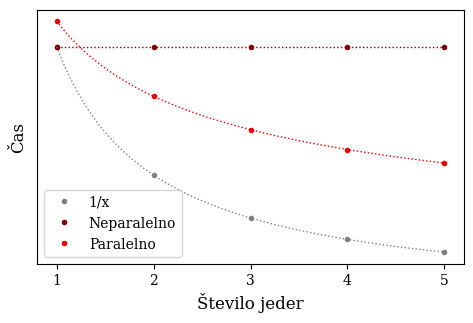
\includegraphics[width=6cm]{slike/cilj-casovne-zahtevnosti-paralelizacije.png}
        \label{fig:cilj-casovne-zahtevnosti-paralelizacije}
    \end{figure}
\end{frame}


\begin{frame}{Paralelizacija v funkcijskih jezikih}
    \begin{itemize}
        \item Funkcijski jeziki: omogočajo enostavno paralelizacijo.
        \item Visoka stopnja abstrakcije: zmanjšuje napake.
        \item Imutabilnost: preprečuje težave z dostopom do spremenljivk.
        \item Težave paralelizacije, ki s funkcijskimi jeziki izginejo: Spremenljivost spremenljivk, stranski učinki, težave s paralelizacijo pomnilnika.
        \item Že implementirane funkcijske knjižnice za paralelizacijo (Haskell: Graphalyze, Scali: GraphX, F\#: Alea.cuBase).
    \end{itemize}
\end{frame}

\begin{frame}{Grafovski algoritmi}
    \begin{itemize}
        \item Grafi: pomembna struktura v računalništvu.
        \item Grafovski algoritmi: rešujejo probleme, povezane z grafi.
        \item Primeri: Najkrajša pot, raziskovanje grafa, iskanje krepko povezanih komponent, algoritmi za posebne grafe (npr. DAG-e).
    \end{itemize}
\end{frame}


\section{Paralelno računanje Fibonaccijevega zaporedja}

\begin{frame}[fragile]
    \frametitle{Izračun Fibonaccijevih števil}
    \begin{itemize}
        \item Naivna implementacija Fibonaccijeve funkcije v jeziku OCaml:
    \begin{verbatim}
    let rec fib n =
      if n < 2 then 1
      else fib (n-1) + fib (n-2)
    \end{verbatim}
        \item Cilj: Pohitriti implementacijo, ki sicer potrebuje $O(n^2)$.
    \end{itemize}
\end{frame}
    

\begin{frame}
    \frametitle{Pregled knjižnice Domainslib}
    \begin{itemize}
        \item \href{https://github.com/ocaml-multicore/domainslib}{Knjižnica Domainslib} - sočasna programska knjižnica za OCaml, ki omogoča paralelizacijo na procesorskem nivoju:
        \begin{itemize}
            \item Domene - niti, ki nam zagotavljajo sočasnost v OCaml-u. Nova domena: ~\texttt{Domainslib.make}
            \item Paralelne naloge - naloge, ki se izvajajo v domenah. Nova naloga se ustvari z ~\texttt{Domainslib.Task.async} ter počaka z ~\texttt{Domainslib.Task.await}
            \item Vzorci vzporednega računanja: ~\texttt{Domainslib.Parallel.map}, ~\texttt{Domainslib.Parallel.For}, \dots
            \item Sinhronizacijski mehanizmi: ~\texttt{Domainslib.Sync}, ~\texttt{Domainslib.Sync.Event}, \dots
            \item Izravnavanje obremenitve med domenami
        \end{itemize}
    \end{itemize}
\end{frame}

\begin{frame}[fragile]
    \frametitle{Paralelizacija izračuna Fibonaccijevih števil}
    \begin{itemize}
        \item Težava: Preveliko število vzporednih niti
        \item Ideja: Paralelizacija najbolj časovno zahtevnih delov kode
        \item Uporaba Domainslib za paralelizacijo v OCamlu (implementacija na tem naslovu 
        \href{https://github.com/tjazerzen/parallelisation-of-graph-algorithms-in-functional-programming-languages/blob/parallel_fibonacci/playground/graph/fib.ml}{tem naslovu}):
    \begin{verbatim}
module T = Domainslib.Task
let rec fib n = 
  if n < 2 then 1 
  else fib (n - 1) + fib (n - 2)
let rec fib_par pool n =
  if n <= 38 then fib n
  else
  let a = T.async pool (fun _ -> fib_par pool (n-1)) in
  let b = T.async pool (fun _ -> fib_par pool (n-2)) in
  T.await pool a + T.await pool b
    \end{verbatim}
    \end{itemize}
\end{frame}

\begin{frame}
    \frametitle{Čas izračuna $fib(n)$ v odvisnosti od števila domen}
    \begin{figure}
        \centering
        \caption{Čas izračuna 43. Fibonaccijevega števila v odvisnosti od števila domen}
        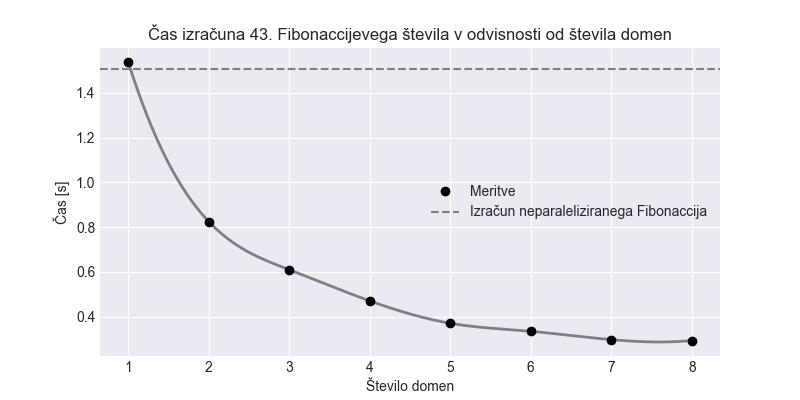
\includegraphics[width=9cm]{slike/fib_par_v_odvisnosti_od_domen.jpg}
        \label{fig:fib_par_v_odvisnosti_od_domen}
      \end{figure}
\end{frame}

\begin{frame}
    \frametitle{Čas izračuna $fib(n)$ pri fiksnem številu domen v odvisnosti od $n$}
    \begin{figure}
        \centering
        \caption{Čas izračuna Fibonaccijevih števil v odvisnosti od zahtevanega Fibonaccijevega števila: Paralelno in neparalelno}
        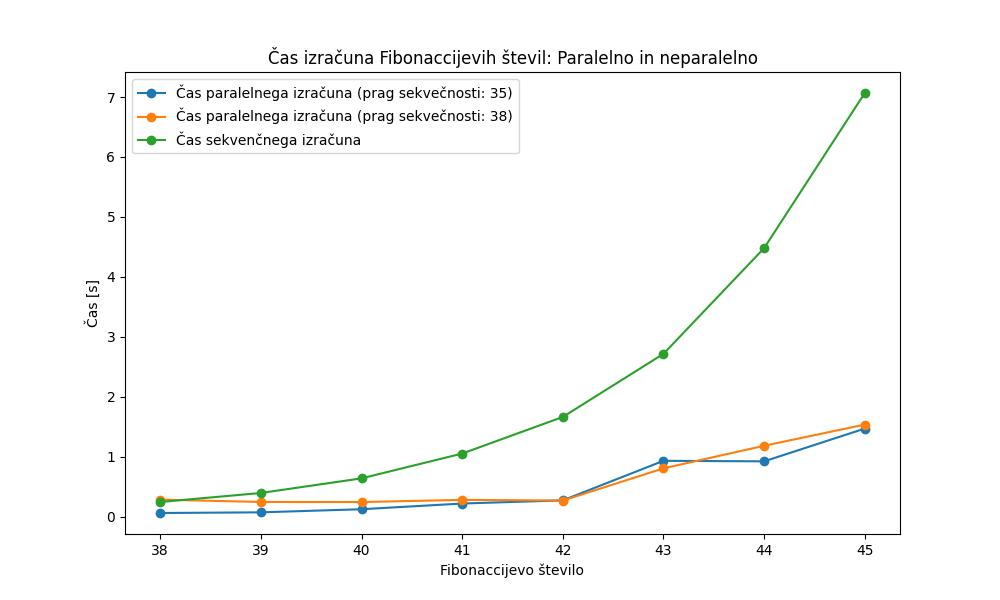
\includegraphics[width=9cm]{slike/fib_par_v_odvisnosti_od_n.jpg}
        \label{fig:fib_par_v_odvisnosti_od_n}
      \end{figure}
\end{frame}
    
    

\section{Prestavitev grafa v funkcijskem jeziku}

\begin{frame}{Načini predstavitve grafa}
    V svoji diplomski grafe predstavim na dva načina:
    \begin{enumerate}
    \item Imperativna predstavitev grafa (spr. podatkovne strukture): Vozlišča hranimo v tabeli, povezave pa v matriki sosednosti
    \item Funkcijska predstavitev grafa (nespr. podatkovne strukture): \texttt{map}, \texttt{IntSet}, \texttt{NodeMap}, \dots
    \end{enumerate}
\end{frame}


\begin{frame}[fragile]
    \frametitle{Imperativna predstavitev grafa}
    \begin{verbatim}
    type 'a node = {
      created_time: float;
      id: int;
      value: 'a;
    }
    
    type 'a graph = {
      nodes: ('a node Option.t) Array.t;
      adjacency_list: IntSet.t Array.t;
      is_directed: bool;
      node_count: int;
    }
    \end{verbatim}
    \href{https://github.com/tjazerzen/parallelisation-of-graph-algorithms-in-functional-programming-languages/blob/predstavitev_grafa_z_arrayi_ter_mnozicami/playground/graph/graph.ml}{[link do implementacije]}.
\end{frame}

\begin{frame}[fragile]
    \frametitle{Funkcijska predstavitev grafa}
\begin{verbatim}
module Node = struct
    type elt = int
    type t = { id : int; value : elt }
    ...
end

module Graph = struct
    type t = {
    edges : NodeSet.t NodeMap.t;
    directed : bool;
    }
    ...
end
    \end{verbatim}
        
    \href{https://github.com/tjazerzen/parallelisation-of-graph-algorithms-in-functional-programming-languages/blob/master/playground/graph/graph.ml}{[link do implementacije]}.
\end{frame}

\begin{frame}
    \frametitle{Prednosti in slabosti}
    Prednosti in slabosti obeh predstavitev:
    \begin{itemize}
    \item Imperativna predstavitev: Bolj znana ter intuitivna, tipično hitrejša za večje grafe, vendar v nasprotju s filozofijo funkcijskega programiranja.
          Težja za paralelno izvajanje.
    \item Funkcijska predstavitev: V skladu z vzorci funkcijskega programiranja, lažje za paralelno izvajanje.
    \end{itemize}
\end{frame}

\begin{frame}{Primerjava časovnih zahtevnosti grafovskih operacij med implementacijama}

    \begin{table}
      \centering
      \footnotesize
      \begin{tabular}{|c|c|c|}
      \hline
      \textbf{Operacija / implementacija} & \textbf{Spremenljive p.s.} & \textbf{Nespremenljive p.s.} \\ \hline
      \textbf{Dodajanje vozlišča} & $O(\log |V|)$ & \underline{$O(1_{amort.})$} \\ \hline
      \textbf{Odvzemanje vozlišča} & $O(|V| \log |V|)$ & \underline{$O(|V|)$} \\ \hline
      \textbf{Dodajanje povezave} & \underline{$O(\log |V|)$} & $O(|V| + |E|)$ \\ \hline
      \textbf{Odvzemanje povezave} & \underline{$O(\log |V|)$} & \underline{$O(\log |V|)$} \\ \hline
      \textbf{Soseščina($u$)} & \underline{$O(deg_Gu + \log |V|)$} & \underline{$O(deg_Gu + \log |V|)$} \\ \hline
      \end{tabular}
      \caption{Primerjava časovnih kompleksnosti operacij na grafu med različnima implementacijama. Podčrtana je tista 
      implementacija, ki je za dano metodo boljša.}
      \label{tab:primerjava_casovnih_kompleksnosti_operacij_na_grafu_med_razlicnima_implementacijama}
    \end{table}
    
\end{frame}
    

\section{Paralelno iskanje v širino (PBFS)}

\begin{frame}{Splošno: Algoritem BFS}
    \begin{figure}
        \centering
        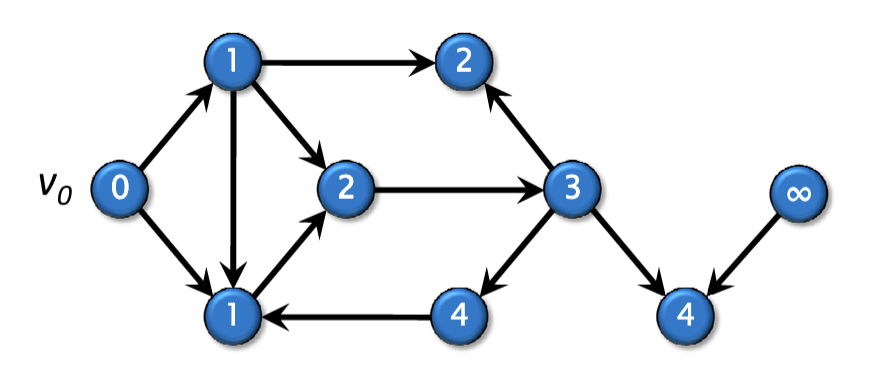
\includegraphics[width=6cm]{slike/parallel_bfs/pbfs_graph_example.png}
        \label{fig:pbfs_graph_example}
    \end{figure}
    Naloga: Ob danem grafu $G=(V, E)$ in začetnem vozlišču $s \in V$ najdemo najkrajše poti od $s$ do vseh ostalih vozlišč.
\end{frame}

\begin{frame}{Algoritem BFS}
    \begin{algorithm}[H]
      \SetAlgoLined
      \DontPrintSemicolon
      \SetKwFunction{FMain}{BFS}
      \label{alg:non_parallel_bfs}
      \FMain{$G,s$}{
        $Q \gets \emptyset$\;
        $Q.\text{enqueue}(s)$\;
        $visited \gets \emptyset$\;
        $visited.\text{add}(s)$\;
        \While{$Q \neq \emptyset$}{
          $u \gets Q.\text{dequeue}()$\;
          \For{$v \in G.\text{adj}(u)$}{
            \If{$v \notin visited$}{
              $visited.\text{add}(v)$\;
              $Q.\text{enqueue}(v)$\;
            }
          }
        }
      }
    \end{algorithm}
  \end{frame}
  
\begin{frame}{Intuicija za delovanjem algoritma BFS}
    \begin{figure}
        \centering
        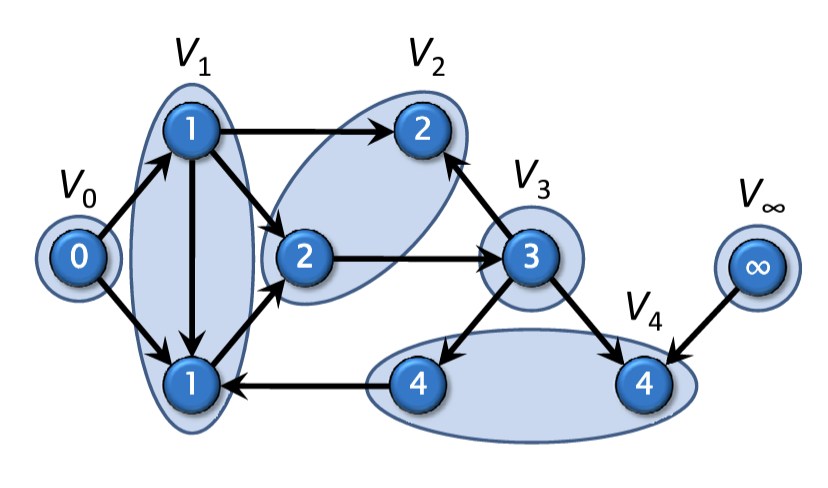
\includegraphics[width=9cm]{slike/parallel_bfs/pbfs_graph_by_levels.png}
        \label{fig:pbfs_graph_example}
    \end{figure}
\end{frame}

\begin{frame}{Paralelni algoritem iskanja v širino}
    \begin{itemize}
        \item Ideja: Vozlišča, ki jih obiskujemo na istih nivojih so neodvisna, zato jih lahko obiskujemo hkrati.
        \item Za vsak nivo $i$ ustvarimo novo domeno, ki obiskuje vozlišča na nivoju $i$.
    \end{itemize}
    \href{https://github.com/tjazerzen/parallelisation-of-graph-algorithms-in-functional-programming-languages/blob/parallel_BFS/playground/graph/bfs.ml}{[link do implementacije]}.
\end{frame}


\end{document}
